%
% File paper.tex
% Copyright © 2018 Max Meldrum

\documentclass[11pt]{article}
\usepackage{acl2015}
\usepackage{times}
\usepackage{url}
\usepackage{latexsym}
\usepackage{natbib}
\usepackage{graphicx}
\usepackage{pdfpages}


\usepackage[noend]{algpseudocode}
\usepackage{amsmath}
\usepackage{algorithm}
\usepackage{pifont}
\usepackage{float}

%\setlength\titlebox{5cm}

% You can expand the titlebox if you need extra space
% to show all the authors. Please do not make the titlebox
% smaller than 5cm (the original size); we will check this
% in the camera-ready version and ask you to change it back.


\title{Hello World: Special Edition}

\author{Max Meldrum \\
{\tt max@meldrum.se}}

\makeatletter
\def\BState{\State\hskip-\ALG@thistlm}
\makeatother

\date{}

\begin{document}
\maketitle
\begin{abstract}
Since being introduced in the book "The C Programming Language", Hello World has become the typical way of how people are introduced to the world of programming. We observe that the classical approach is conservative, all characters are displayed solely through one programming language. In this paper, we propose an improved version which enables the execution to transpire through multiple languages.
\end{abstract}

\section{Introduction}
Instructing the computer to display text on the screen is the most common first program that any developer will encounter. The concept of Hello World became popular through\cite{Kernighan:1988:CPL:576122}. Many years has past since its introduction, and still there has not been any further research into the language exposure aspect of Hello World.
\newline{}\newline{}
The remainder of the paper introduces the special edition algorithm (Section 2), dissects the performance and language exposure (Section 3), discusses next generation Hello World programs (Section 4) and draws the conclusion (Section 5).

\section{Algorithm}
In our reference implementation\footnote{https://github.com/Max-Meldrum/hello-world-special-edition/}, we elected to go for "Hello World!" rather than "Hello, World!". In total, including the white space, we have 12 characters. It is possible to connect any amount of languages. However, it is not guaranteed that the 12 selected languages will be unique. The algorithm will pick randomly from a basket.
\newline{}\newline{}
Special Edition can be understood by describing its two phases. In phase 1 (initialization phase), there is a confirmation step that compilers of the chosen languages are available. If the examination goes through without any issues, all languages are inserted in to a List, which is then used to generate another list with 12 random languages. One important thing to note is that as long as you have one language available, the algorithm will be able to run. If Python, C and Java are selected, the algorithm will simply pick randomly from the three until it has a total of 12.
\newline{}\newline{}
A prerequisite for Special Edition is the capability of executing system calls. Executor's (see 2.1) utilises system calls to pass on the next task to the Controller (see 2.2).

\begin{algorithm}[H]
\caption{Initialization Phase}
\label{Special Edition}
\begin{algorithmic}[1]
\Procedure{GenerateLanguages}{}
\State $N\gets 12$
\State $L\gets Languages$
\For{$N$ iterations}
	\State $S\gets Random(L)$
\EndFor
\State \textbf{return} S
\EndProcedure
\end{algorithmic}
\end{algorithm}

\subsection{Executor}
The Executor system has two tasks. PartialPrint and Notify. The former checks if the given character position is valid, if it is, it then prints the character that corresponds to the position. The latter reviews the current position and decides whether to pass on the task via the Controller or exit the system.
\newline{}\newline{}
For the final output to be outputted correctly, the buffered stdout has to be flushed after every print operation.
\vfill
\begin{algorithm}[H]
\caption{Executor Algorithm PP}
\label{Special Edition}
\begin{algorithmic}[t]
\Procedure{PartialPrint(pos)}{}
\If{$pos == 0$}
	\State print "H"
\ElsIf{$pos == 1$} 
	\State print "e"
\ElsIf{$pos == 2$}
	\State print "l" 
\ElsIf{$pos == 3$}
	\State print "l"
\ElsIf{$pos == 4$}
	\State print "o"
\ElsIf{$pos == 5$}
	\State print "\texttt{\char`\ }"
\ElsIf{$pos == 6$}
	\State print "W"
\ElsIf{$pos == 7$}
	\State print "o"
\ElsIf{$pos == 8$}
	\State print "r"
\ElsIf{$pos == 9$}
	\State print "l" 
\ElsIf{$pos == 10$}
	\State print "d"
\ElsIf{$pos == 11$}
	\State print "!"
\ElsIf{$pos == 12$}
	\State print "\texttt{\char`\\n}"
\EndIf
\EndProcedure
\end{algorithmic}
\end{algorithm}

\begin{algorithm}[H]
\caption{Executor Notify}
\label{Special Edition}
\begin{algorithmic}[t]
\Procedure{Notify(pos, nlangs)}{}
\If{pos \texttt{\char`\>=} 0 and pos \texttt{\char`\<} 12} \State $target\gets nlangs.head$
	\State $executors\gets nlangs.dropHead$	
	\State Controller(target,  pos+1, executors)
\Else
	\State shutdown() 
\EndIf
\EndProcedure
\end{algorithmic}
\end{algorithm}
\raggedbottom
\subsection{Controller}
The controller acts as a bridge between Executor's. After an Executor has printed a character, it notifies the controller of the next target language, position and the list that contains the Executor order. With this information, the bridge acts like a proxy and runs the new Executor. The controller can be implemented in any language that has basic features. A shell script is used in the reference implementation.
\vfill
\raggedbottom

\begin{algorithm}[H]
\caption{Controller Algorithm}
\label{Special Edition}
\begin{algorithmic}[2]
\Procedure{Bridge(target, pos, nlangs)}{}
	\State Execute(Target).with(pos, nlangs)
\EndProcedure
\end{algorithmic}
\end{algorithm}

\section{Evaluation}
The traditional Hello World program outpeforms the Special Edition version in runtime performance as there will be delays between each Executor instance. However, what we are interested in is the maximum amount of languages that can be connected.
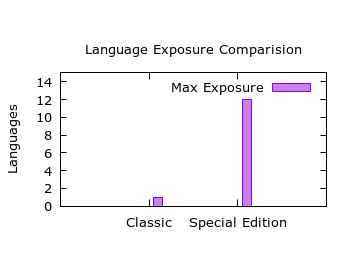
\includegraphics[scale=0.65]{img/exposure.png}


\section{Future Work}
Special Edition runs locally on the computer. One could improve the system to be capable of executing Hello World in a peer-to-peer fashion. A peer would be able to act as an Executor and a Controller. This would increase the language exposure immensely as the more computers that are connected to the network, the bigger chance we have of being exposed to more languages.

\section{Conclusion}
The traditional approach to Hello World is only executed with one language in mind. In this paper, we describe an improved version named Special Edition which supports the execution to occur through multiple languages. We draw the conclusion that our version increases the level of language exposure at cost of performance. We believe that this is just the first step into the next generation of Hello World programs.

%\section*{Acknowledgments}


\bibliography{references}
\bibliographystyle{unsrt}

\end{document}
